%%%%%%%%%%%%%%%%%%%%%%%%%%%%%%%%%%%%%%%%%%%%%%%%%%%%%%%%%%%%%%%%%%%%%%%%%%%%%%%%
%2345678901234567890123456789012345678901234567890123456789012345678901234567890
%        1         2         3         4         5         6         7         8

\documentclass[letterpaper, 10 pt, conference]{ieeeconf}  % Comment this line out
                                                          % if you need a4paper
%\documentclass[a4paper, 10pt, conference]{ieeeconf}      % Use this line for a4
                                                          % paper
\IEEEoverridecommandlockouts                              % This command is only
                                                          % needed if you want to
                                                          % use the \thanks command
%\overrideIEEEmargins
% See the \addtolength command later in the file to balance the column lengths
% on the last page of the document

% The following packages can be found on http:\\www.ctan.org
\usepackage{cite}
\usepackage{amsmath,amssymb,amsfonts}
\usepackage{algorithmic}
\usepackage[ruled,vlined,linesnumbered]{algorithm2e}
\usepackage{graphicx}
\usepackage{textcomp}
\usepackage{xcolor}
\usepackage{flowchart}
\usetikzlibrary{shapes,arrows}

\title{\LARGE \bf
Outlier Detection for ARM Data
}

\author{Yuping Lu$^{1}$, Jitendra Kumar$^{2}$, Nathan Collier$^{2}$ and Michael A. Langston$^{1}$% <-this % stops a space
\thanks{$^{1}$University of Tennessee, Knoxville, TN, USA}%
\thanks{$^{2}$Oak Ridge National Laboratory, Oak Ridge, TN, USA}%
}

\begin{document}
\maketitle
\thispagestyle{empty}
\pagestyle{empty}

%%%%%%%%%%%%%%%%%%%%%%%%%%%%%%%%%%%%%%%%%%%%%%%%%%%%%%%%%%%%%%%%%%%%%%%%%%%%%%%%
\begin{abstract}

The Atmospheric Radiation Measurement (ARM) Data Center collects data from either permanent or mobile facilities around the globe. These data are then ingested and used to create high level scientific products which requires great accuracy. Multiple methods are available to detect these outliers from ARM time series data. As outliers are common in the collected data which could be either an instrument failure or extreme weather event, Pearson correlation coefficient was first examined to measure the pairwise correlations between variables. New version of Singular Spectrum Analysis (SSA) was also introduced to detect outliers. K-means was applied in a different manner to filter out the abnormal records as well. Pearson correlation coefficient, SSA and K-means methods were later combined together as a whole framework to track down these outliers. Compared to the current data quality reports stored in the DQR database, our results showed this framework is promising.

\end{abstract}


%%%%%%%%%%%%%%%%%%%%%%%%%%%%%%%%%%%%%%%%%%%%%%%%%%%%%%%%%%%%%%%%%%%%%%%%%%%%%%%%
\section{Introduction}
The Atmospheric Radiation Measurement (ARM) user facility was founded by the U.S. Department of Energy (DOE) in 1989 \cite{ARM}. Since then, its aim is to be the platforms for the observation and study of Earth's climate. Huge ARM datasets are collected from instruments deployed in different ground stations across the globe \cite{stokes1994atmospheric}. ARM Data Center is responsible for ingesting these collected data and creates high level scientific data products for distribution and the improvement of global climate models (GCMs) \cite{gaustad2014scientific}. These high level data products, also called "Value Added Products" (VAPs) are highly dependent on the correctness of the raw data. Thus it is crucial to detect those outliers in the raw data and correct them.

% The general definition of outlier detection and their types.
Outlier detection, also called anomaly detection or intrusion detection, is a common task in many application domains which include time series data, streaming data, distributed data, spatio-temporal data, and network data \cite{gupta2014outlier}. Common techniques for outlier detection include signal processing, classification, clustering, nearest neighbor, density, statistical, information theory, spectral decomposition, and visualization. Among all these techniques, time series data outlier detection and temporal network outlier detection are especially useful for ARM data.

% Outlier detection for time series data
Outlier detection in time series data was first studies by Fox in 1972 \cite{fox1972outliers}. Common types of outlier are additive outliers, level shifts, temporary changes, and innovative outliers. One common approach is the discriminative method which is based on a similarity function. For example, normalized longest common subsequence (NLCS) is a similarity measurement widely used in the field of data mining \cite{budalakoti2009anomaly, chandola2008comparative, sequeira2002admit}. Commonly used clustering methods such as K-means \cite{macqueen1967some}, dynamic clustering \cite{sequeira2002admit}, single-linkage clustering \cite{portnoy2001intrusion}, Principal component analysis (PCA) \cite{gupta2013context}, and self-organizing map (SOM) \cite{gonzalez2003anomaly} are also popular. The choice of the clustering algorithm depends on the problem itself as each has different size and complexity. Three unsupervised parametric models, Finite state automata (FSA), Markov models, and Hidden Markov Models (HMMs), are often seen in outlier detection as well. An outlier is detected if the FSA in the current state couldn't reach the final state \cite{chandola2008comparative}. The history size in the Markov model could be either fixed or flexible. HMMs are easy to interpret but not function well with big datasets \cite{chandola2008comparative}. Researchers also tried supervised methods such as neural networks \cite{dasgupta2000comparison}, Support vector machines (SVMs) \cite{li2006motion}, and decision tree \cite{kang2005learning} to detect outliers.

% window based methods
Different from the methods mentioned above, window-based detection is breaking the time series data into overlapping subsequences with fixed window size \cite{cheboli2010anomaly}. Each window is assigned an anomaly score, and then a final score for the times series data by aggregating the window scores. Subspace based analysis for univariate time series data is similar to window-based detection. The subspace based transformation is to convert a univariate time series into a multivariate time series with fixed window size. It then transforms the multivariate time series back to univariate time series. Singular Spectrum Analysis is a good example of this idea \cite{golyandina2013singular}.

% Outliers detection for temporal networks: graph, community etc. 
Temporal data is a broad concept which include commercial transactions, sensor data, astronomy data, computer network traffic, medical records, judicial records, social network data and many others. Many challenges exist for outlier detection for temporal data. First, the algorithm or model needs to understand the properties of the data and network. Second, the temporal data has space and time dimensions which make it complex to analysis. Third, its scale is massive and efficient algorithm is crucial for fast outlier detection. One common problem for temporal data is to detect outlier graph snapshots from a series graph snapshots in temporal networks. Spearman’s correlation coefficient is a good candidate for such problem. It is the rank correlation between two sorted lists of graph vertices which are ordered by PageRank or other properties \cite{papadimitriou2010web}. Similar to Spearman’s correlation coefficient, Pearson correlation coefficient is also commonly used. Jaccard similarity is the size of intersection vertex set divided by the size of union vertex set \cite{jay2012systematic}. Graph edit distance describes the necessary changes to make graph $G_1$ isomorphic to graph $G_2$. It can defined as $d(G_1, G_2) = |V_{G_1}| + |V_{G_2}| - 2|V_{G_1} \cap V_{G_2}| + |E_{G_1}| + |E_{G_2}| - 2|E_{G_1} \cap E_{G_2}|$ \cite{papadimitriou2010web}. The spectral distance is the difference between the adjacency spectrum of graph $G_1$ and $G_2$, written as $\sigma(G_1, G_2) = \displaystyle\sum_{i=1}^{n}|\lambda_i(G_1) - \lambda_i(G_2)|$ \cite{jovanovic2012spectral}. Entropy distance is defined by the entropy-like measurement between two graphs \cite{pincombe2005anomaly}. All these metrics are also common seen in temporal network outlier detection.

% Application of outlier detection environmental sensor data
Many applications are available for temporal outlier detection, especially environmental sensor data. Birant et al \cite{kut2006spatio} discovered locations with high wave heights are outliers while studying the wave height values from the east of the Mediterranean Sea, the Marmara Sea, the Black sea, and the Aegean Sea. Hill et al \cite{hill2007real, hill2010anomaly} filtered out measurement errors in the wind speed data stream from WATERS Network Corpus Christi Bay testbed with dynamic Bayesian networks. Drosdowsky et al \cite{drosdowsky1993analysis} found anomalies from Australian district rainfall using rotated PCA. Wu et al. \cite{wu2010spatio} detected precipitation outlier events while working on South American precipitation data set. Sun et. al \cite{yuxiang2005detecting} extracted locations which always have different temperature from their surroundings by exploring the South China area dataset from 1992 to 2002.

\section{Datasets}
ARM data are stored in Network Common Data Form (NetCDF) format which is self-describing and machine-independent \cite{rew1990netcdf, NetCDF}. NetCDF format also has good performance and data compression. It is commonly used to handle scientific data, especially those from the climatology, meteorology, oceanography and GIS projects. ARM data is publicly available and can be downloaded from ARM Data Archive (http://www.archive.arm.gov). Kinds of raw data are stored in ARM Data Center. It ranges from \textit{Atmospheric Profiling} to \textit{Satellite Observations}. All these data are measured at different locations using different instruments. Each instrument may only work on a specified time range. For the raw NetCDF dataset collected from each instrument, it contains multiple variables. 

\begin{table}[ht]
\caption{SGPMET datasets tested}
\label{tab:datasets}
\centering
\begin{tabular}{|l|c|c|c|c|c|c|c|c|}
\hline
Instrument & E1 & E3 & E4 & E5 & E6 & E7\\
Begin Year & 1996 & 1997 & 1996 & 1997 & 1997 & 1996\\
End Year & 2008 & 2008 & 2010 & 2008 & 2010 & 2011\\
\hline
Instrument & E8 & E9 & E11 & E13 & E15 & E20\\
Begin Year & 1994 & 1994 & 1996 & 1994 & 1994 & 1994\\
End Year & 2008 & 2017 & 2017 & 2017 & 2017 & 2010\\
\hline
Instrument & E21 & E24 & E25 & E27 & E31 & E32\\
Begin Year & 2000 & 1996 & 1997 & 2004 & 2012 & 2012\\
End Year & 2017 & 2008 & 2001 & 2009 & 2017 & 2017\\
\hline
Instrument & E33 & E34 & E35 & E36 & E37 & E38\\
Begin Year & 2012 & 2012 & 2012 & 2012 & 2012 & 2012\\
End Year & 2017 & 2017 & 2017 & 2017 & 2017 & 2017\\
\hline
\end{tabular}
\end{table}

In this paper, we only tested Surface Meteorology Systems (MET) data collected from the Southern Great Plains (SGP). There were total 24 instruments in SGP area and we chose 5 typical variables which are \textit{temp\_mean}, \textit{vapor\_pressure\_mean}, \textit{atmos\_pressure}, \textit{rh\_mean} and \textit{wspd\_arith\_mean} from multiple variables. Table 1 contains the detail of these datasets. 

\section{Methodology}
We have introduced many kinds of outlier detection method in the first section. We carefully picked three algorithms and tested them on ARM data. We also did necessary preprocessing before running these algorithms. The first level raw data is stored in minute level. It is normalized for pairwise comparison algorithm. Some algorithms may not need so much detail information to extract outliers. Thus we created a second level data by averaging the 1440 minute data points into one day point from the raw data. The second level data can save a lot of running time and is easier for Plotly \cite{plotly} and Matplotlib \cite{Hunter:2007} to visualize. The third level data was especially created for multivariate method by standardization all the 5 variables into the same scale based on the second level data. Below we will talk about each algorithm in detail. 

\subsection{Pearson correlation coefficient} 
Pearson correlation coefficient was first introduced by Karl Pearson\cite{pearson1895note}. It is used to measure the linear correlation between two variables. Pearson correlation coefficient is calculated from the covariance of two variables divided by the multiplication of the standard deviation of those two variables. Thus the value falls in [-1, 1]. If the value is close to -1, it means those two variables are highly negatively related. On the other hand, then the two variables are strongly positively related. If the value is near 0, it means those two variables don't have linear relation. 

\begin{figure*}[ht]
    \centering
    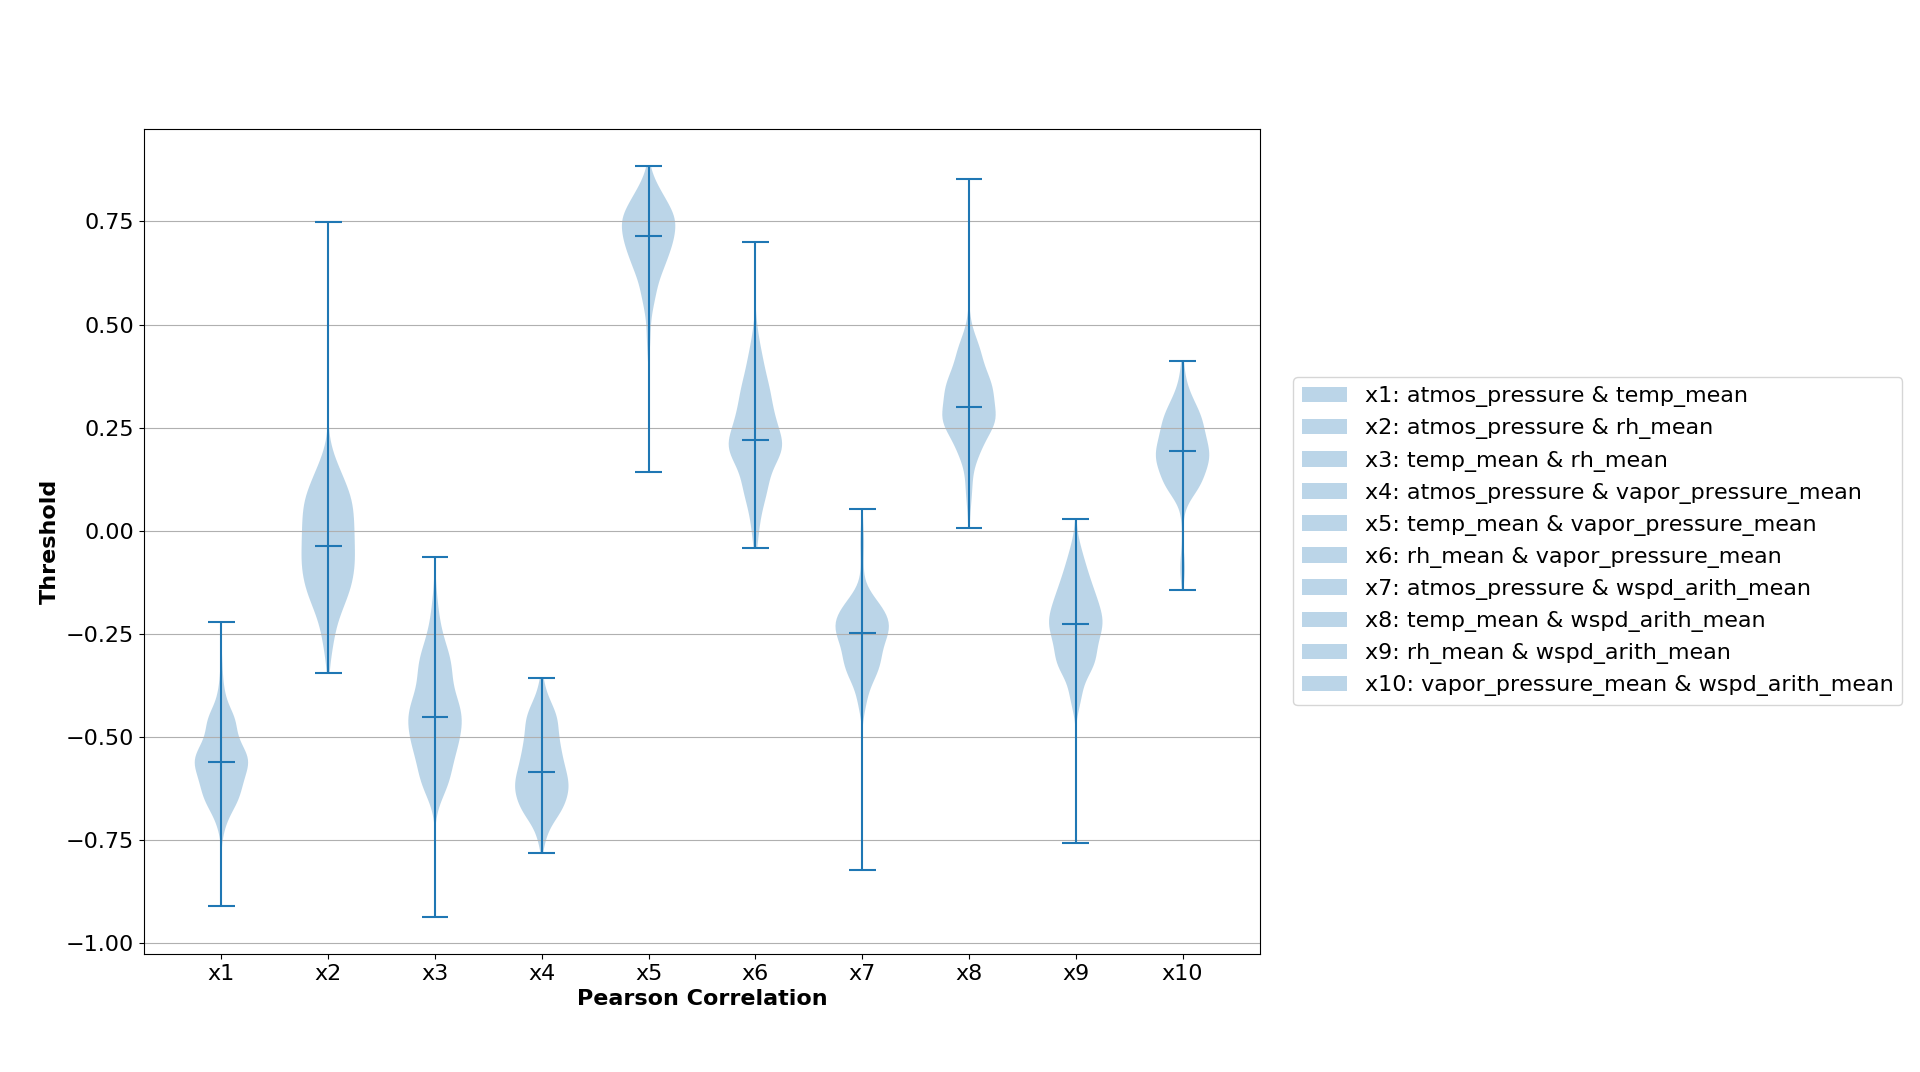
\includegraphics[width=\textwidth]{Spring.png}
    \caption{Violin plot: Spring 5 variables from SGPMET}
    \label{fig:pc}
\end{figure*}

We performed pairwise comparison of the 5 variables using Pearson correlation on all the instruments in a seasonal level. The result in figure 1 makes sense and all the correlations in this violin plot are normally distributed. For example, x5 the Pearson correlation between \textit{temp\_mean} and \textit{vapor\_pressure\_mean} is positively correlated with correlation mean close to 0.75. x1 is negatively correlated with correlation mean close to -0.60. We used this correlation as base knowledge. If a pairwise pearson correlation of two variables from a specific season of a instrument falls out of that range, we treated that seasonal data as outliers.

\subsection{Singular Spectrum Analysis}
Singular Spectrum Analysis (SSA) is a popular method for time series data analysis \cite{golyandina2013singular, golyandina2014basic}. The general idea is to use a subset of the decomposition of trajectory matrix to approximate it. Many applications can be found in \cite{golyandina2013singular}. For example, SSA can be applied to monitor volcanic activity \cite{bozzo2010relationship}. It can also be used to extract trend \cite{alexandrov2008method}. Different from the classic SSA method, we defined our own version of SSA to best work on ARM data. Figure 2 is a demonstration of the workflow of SSA. Below is the formal description of the algorithm.

% SSA workflow
\begin{figure}[ht]
    \centering
    % Define block styles
    \tikzstyle{decision} = [diamond, draw, fill=blue!20, text width=4.5em,text badly centered, node distance=3cm, inner sep=0pt]
    \tikzstyle{block} = [rectangle, draw, fill=blue!20, minimum width=5em, text centered, rounded corners, minimum height=2em]
    \tikzstyle{line} = [draw, -latex']
    \tikzstyle{cloud} = [draw, ellipse,fill=red!20, node distance=3cm, text width=3em, minimum height=2em]
    \begin{tikzpicture}[node distance = 2cm, auto]
        % Place nodes
        \node [block] (init) {\small Embedding};
        \node [block, right of=init, node distance=3cm] (decomp) {\small Decomposition};
        \node [block, below of=decomp] (freq) {\small Finding Dominant Frequency};
        \node [block, below of=freq] (period) {\small Converting Periodicity into Frequency};
        \node [block, below of=period] (approx) {\small Approximation};
        \node [block, left of=approx, node distance=3cm] (re) {\small Reconstruction};
        % Draw edges
        \path [line] (init) -- (decomp);
        \path [line] (decomp) -- (freq);
        \path [line] (freq) -- (period);
        \path [line] (period) -- (approx);
        \path [line] (approx) -- (re);
    \end{tikzpicture}
    \caption{Flowchart of SSA}
    \label{fig:pcs}
\end{figure}

\begin{figure*}[ht]
    \centering
    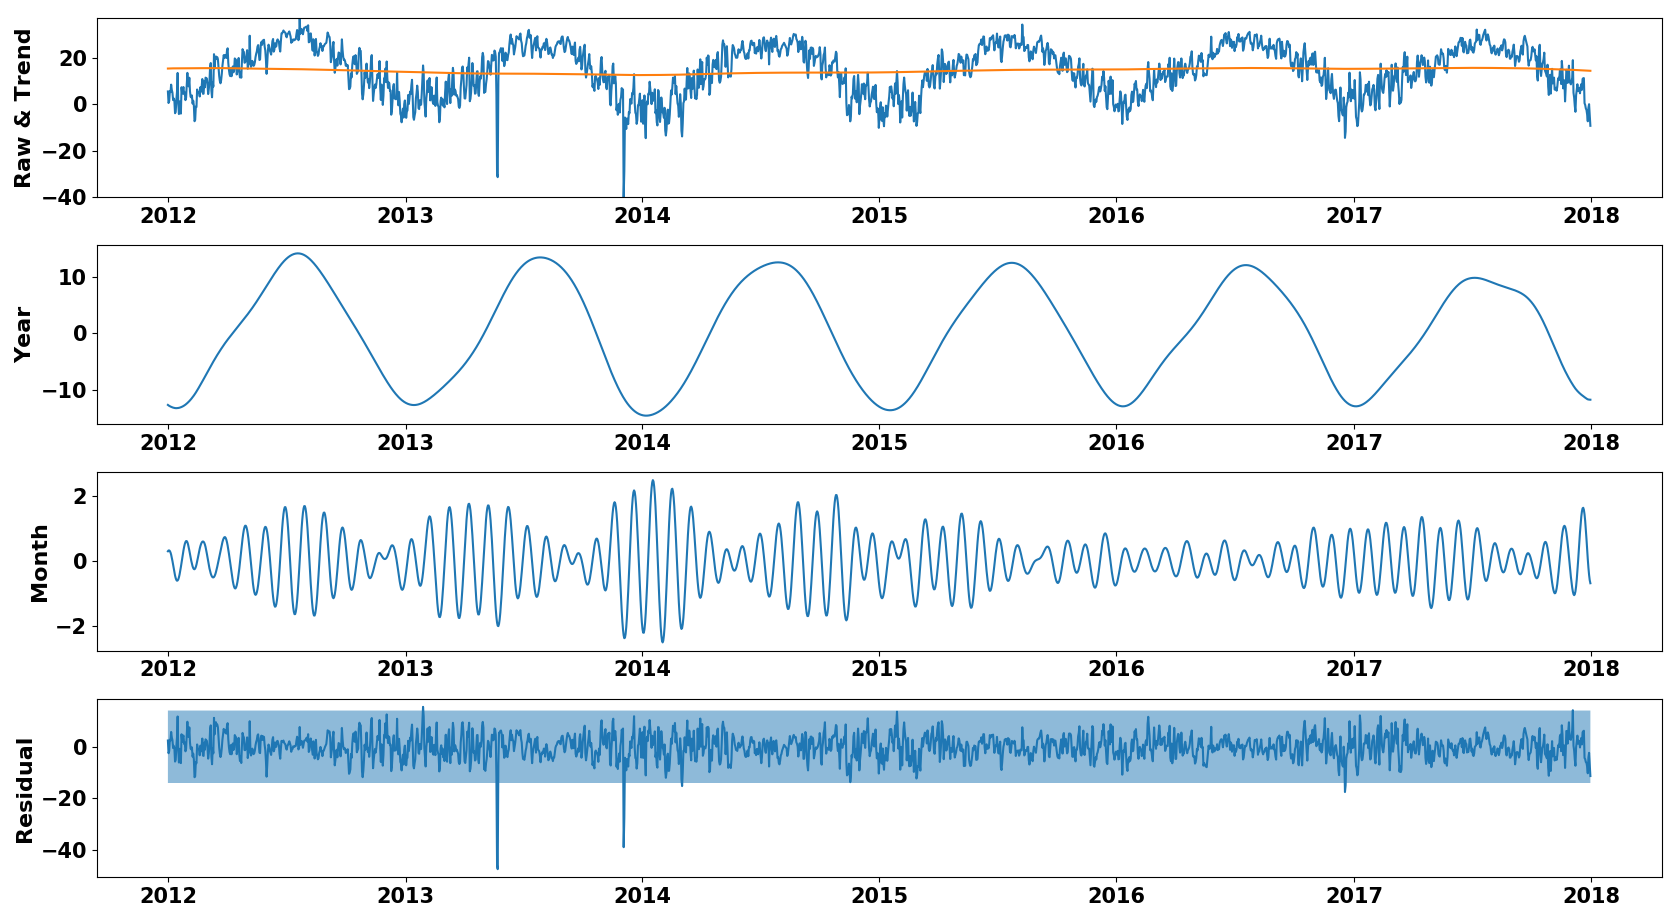
\includegraphics[width=\textwidth]{E33.png}
    \caption{Example of SSA application on ARM data. The full decomposition of \textit{temp\_mean} data from instrument E33.}
    \label{fig:ssa}
\end{figure*}

% SSA algorithm description
% Needs Nate's help, especially step 3. Not sure how to describe this step accurately.
Assume we have an ARM time series data Y of length T.
\begin{align*}
Y =(y_1,\ \ldots,\ y_T)
\end{align*}
Here $T > 2$ and $y_i$ is not empty. Let $L\ (1 < L \leq T/2)$ be the window size and $K = T - L + 1$. In general, the algorithm contains two main parts: decomposition and reconstruction.

1) The first step is to form trajectory matrix \textbf{X} from vector Y by embedding subsets of Y. These subsets of Y $X_i$ are lagged vectors of length L.  
\begin{align*}
X_i = (y_i,\ \ldots,\ y_{L+i-1})^T \quad (1 \leq i \leq K) \\
\mathbf{X} = [X_i,\ \ldots,\ X_K] 
\end{align*}
Thus the trajectory matrix is
\begin{equation}
\mathbf{X} = (x_{ij})_{i,j=1}^{L,K}  = \left(\begin{IEEEeqnarraybox*}[][c]{,c/c/c/c/c,}
y_1 & y_2 & y_3 & \ldots & y_K\\
y_2 & y_3 & y_4 & \ldots & y_{K+1}\\
y_3 & y_4 & y_5 & \ldots & y_{K+2}\\
\vdots & \vdots & \vdots & \ddots & \vdots\\
y_L & y_{L+1} & y_{L+2} & \ldots & y_T
\end{IEEEeqnarraybox*}\right)
\end{equation}
where $x_{ij} = y_{i+j-1}$. We can see from equation 1 that matrix \textbf{X} has equal elements on anti-diagonals and therefore it is Hankel matrix.

2) Assume matrix $\mathbf{S}=\mathbf{XX}^T$, thus we perform the singular value decomposition (SVD) on $\mathbf{S}$. The eigenvalues of S are denoted by $\lambda_1, \ldots, \lambda_L$ in the decreasing order of magnitude $(\lambda_1 \geq \ldots \geq \lambda_L \geq 0)$ and corresponding eigenvectors are denoted by $P_1, \ldots, P_L$. Let $d = rank\ \mathbf{X}$ and $V_i = \mathbf{X}^T P_i / \sqrt{\lambda_i} (i = 1, \ldots, d)$. Thus, the trajectory matrix X can also be written as
\begin{equation}
\mathbf{X} = \mathbf{X_1} + \ldots + \mathbf{X_d}
\end{equation}
where $\mathbf{X_i} = \sqrt{\lambda_i} P_i V_i^T$.

3) In this step, we use Fast Fourier transform (FFT) to find the dominant frequency of each eigenvector \cite{cooley1965algorithm} . Algorithm 1 shows the whole process.

\begin{algorithm}[ht]
\DontPrintSemicolon
\SetAlgoLined
%\KwResult{Dominant frequency of each eigenvector}
\SetKwInOut{Input}{Input}
\SetKwInOut{Output}{Output}
\Input{$\lambda$ of $\mathbf{S}$ and corresponding eigenvectors $\mathbf{P}$}
\Output{Dominant frequency of each eigenvector}
\BlankLine

fftfreq $\leftarrow$ Discrete Fourier Transform sample frequencies\;
fft $\leftarrow$ Discrete Fourier Transform\;
len $\leftarrow$ size of $\lambda$\;
frequencies $\leftarrow$ zero vector of size len\;
fs $\leftarrow$ fftfreq($\lambda$)\;
ix $\leftarrow$ indices that sort fs\;
fs $\leftarrow$ fs[ix]\;
\For{i in range(len)}{
    p1 $\leftarrow$ abs(fft($\mathbf{P}$[:,i]))\;
    ps $\leftarrow$ p1**2\;
    ps $\leftarrow$ ps[ix]\;
    frequencies[i] $\leftarrow$ fs[index of the maximum value in ps]\;
}
\Return abs(frequencies)
\caption{Dominant Frequency Finder}
\end{algorithm}

4) Let G be the vector of user specified periodicity. We then convert G into a vector of targeted frequency TF for the next step. Here 0 is also added to TF. We use M to denote the length of TF.

5) As mentioned in step 2, there are d $\mathbf{X_i}$. The goal is to build an approximation of X by taking a subset of the decomposition $\mathbf{X_i}$. This approximation is formed by taking eigenvectors whose dominant frequency is close to the targeted frequency. Thus we have an approximation matrix $\mathbf{Xt}$ of size $M \times L \times K$.

6) Now we reconstruct the signal $\hat{Y}$ by taking a mean of all the approximations. The generated matrix $\mathbf{Yt}$ with size $M \times T$ can be used to approximate Y.

\begin{equation}
\hat{Y} =  \displaystyle\sum_{i=1}^{M} \mathbf{Yt}[i]
\end{equation}

In this paper, we chose the temp\_mean data from instrument E33 as Y to illustrate SSA. Because SSA requires the time series data to be continuous, we replaced the empty points with the average temp\_mean value for that day in a year. 

We set L = 400 and picked year and month as the periodicity groups G = [365, 30]. Thus TF = [0, 0.00273973, 0.03333333]. The generated matrix $\mathbf{Yt}$ has 3 rows after performing SSA. And $\hat{Y}$ = $\mathbf{Yt}[0]$ + $\mathbf{Yt}[1]$ + $\mathbf{Yt}[2]$. The residual is then extracted from the raw data R = Y - $\hat{Y}$. As $\hat{Y}$ is the approximation which is a "perfect" representation of Y. We then extracted the extreme values from the residual. Those extracted outliers are outliers. Figure 3 is a visualization of the result. The first row is the raw data Y. The orange line $\mathbf{Yt}[0]$ is the trend. As we can see, the trend is pretty flat from 2012 to 2017. The second row and third row are $\mathbf{Yt}[1]$, $\mathbf{Yt}[1]$ respectively. The Year data matches the pattern of the raw data. The last row is the residual. Those peak values outside the blue shaded area are outliers.

\subsection{K-means}
K-means is a partitioning clustering algorithm \cite{macqueen1967some, hartigan1979algorithm}. It starts with the k centroids user specified, and assigns the points to the nearest centroid. Then it computes new k centroids and assign the rest points to these centroids again. The process repeats until it converges. 

% K-means algorithm
\begin{algorithm}[ht]
\DontPrintSemicolon
\SetAlgoLined
%\KwResult{Dominant frequency of each eigenvector}
\SetKwInOut{Input}{Input}
\SetKwInOut{Output}{Output}
\Input{ARM time series data}
\Output{Outliers}
\BlankLine

outliers $\leftarrow \varnothing$\;
df $\leftarrow$ ARM time series data\;
data $\leftarrow$ df['atmos\_pressure','temp\_mean',\
'rh\_mean','vapor\_pressure\_mean','wspd\_arith\_mean']\;
number\_of\_clusters $\leftarrow$ 4\;
clusters $\leftarrow$ K-means(data, number\_of\_clusters)\;
distances $\leftarrow$ Distance between each point and its centroid\;
mean $\leftarrow$ arithmetic mean of distances\;
sigma $\leftarrow$ standard deviation of distances\;
threshold $\leftarrow$ mean + 3 * sigma\;
\For{i in range(size of distances)}{
    \If{distances[i] $>$ threshold}{
        outliers $\leftarrow$ outliers $\cup$ {distances[i]}
    }
}
\Return outliers
\caption{K-means Outlier Detection}
\end{algorithm}

In this paper, we didn't stop after clustering ARM data with K-means. We transformed the generated clusters into a vector of distance between each point and its corresponding centroid. Algorithm 2 describes the whole process. Unlike SSA, we used all the 5 variables mentioned in Datasets section together to extract outliers.

\begin{figure*}[ht]
    \centering
    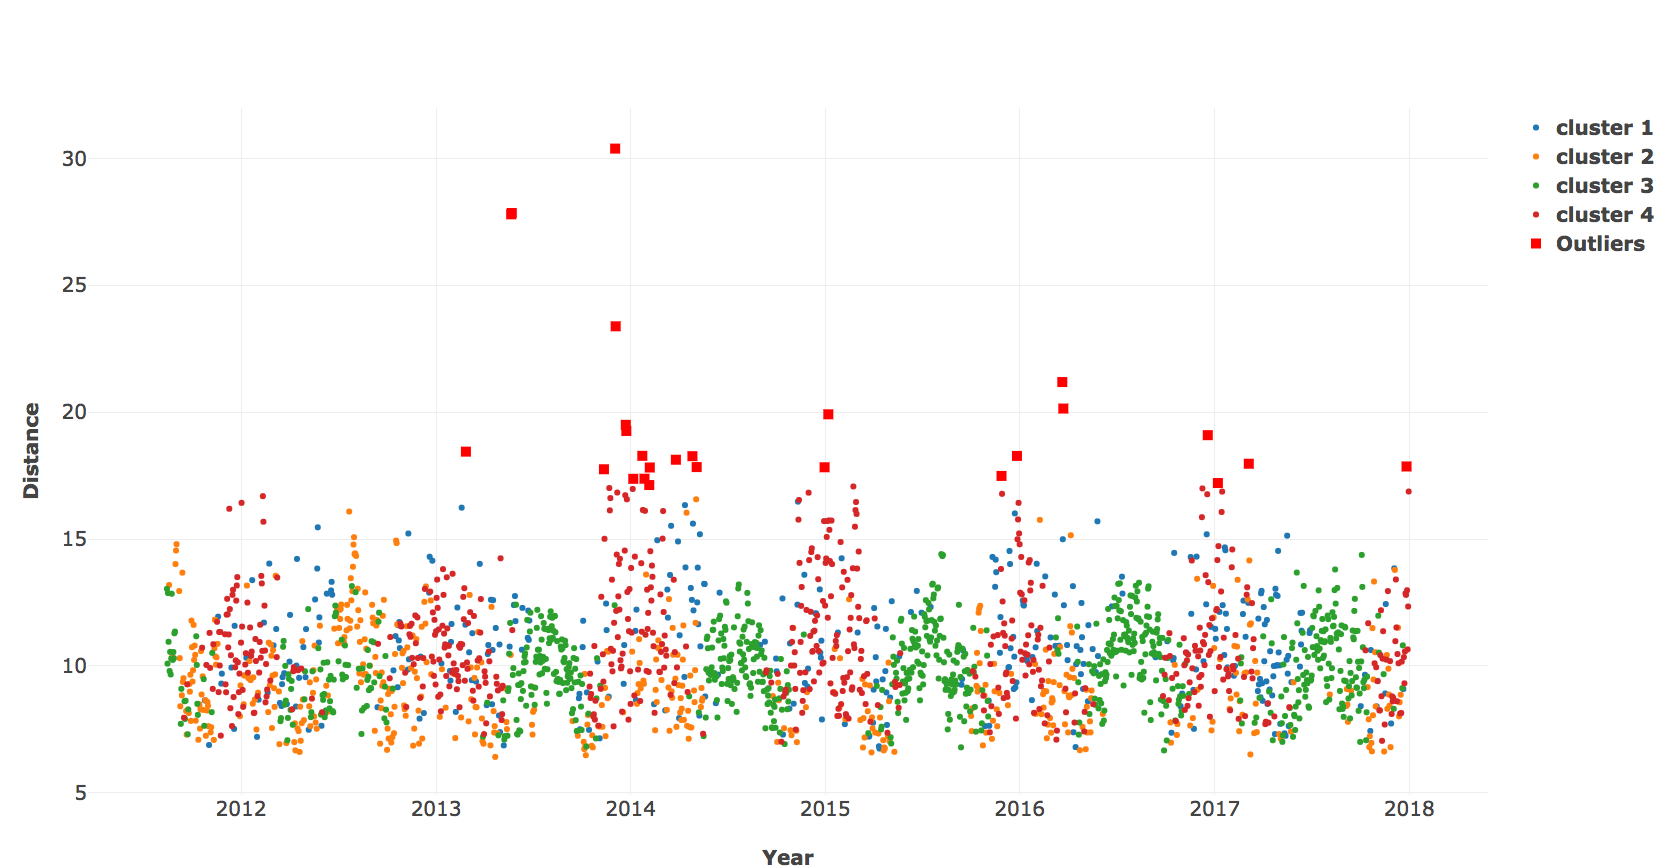
\includegraphics[width=\textwidth]{kmeans.png}
    \caption{Outliers detected using K-means for E33}
    \label{fig:kmeans}
\end{figure*}

Again, we used data from instrument E33 as an example for K-means. Here we set k to 4 as each year has 4 seasons.  Figure 4 visualized the outliers detected from E33. Y axes in this figure is the distance metric. The pattern of these points is close to the raw data.

\section{Results and Discussion}
% mention the usage of python and implementation. % add three sigma rule here.
The three algorithms and visualizations are implemented in Python in this paper. All codes and results are available on GitHub (https://github.com/YupingLu/arm-pearson and https://github.com/YupingLu/arm-ssa). Multiple methods are available to set a threshold for extreme values as outliers. We used the three sigma rule to extract outliers \cite{pukelsheim1994three}. For example, if the distance one point is larger than three sigmas, we treat this point as an outlier in algorithm 2.

% methods drawbacks and advantages
Pearson correlation coefficient is a pairwise comparison method which is used to detect abnormality of correlation between two variables. However if the two variables suddenly change in the same direction, their correlation may still be normal similar to their "supposed" value. It is the same case if only a few outlier points inside a big quantity of data points. As we performed the Pearson correlation coefficient on the seasonal level, it's not possible to track down to the exact day. SSA is a univariate method to detect outliers for each variable in the ARM data. It can quickly catch those high peak and drop points. But it requires the time series data to be continuous with no missing points. K-means is a commonly used multivariate method for clustering. Here we used it for outlier detection. The problem is that the detected outliers could be just one type of variable or multiple types of variable. It's hard to tell which is the case and get the detail for future correction.

% all together as a template
One outlier may only be detected by SSA or Pearson correlation coefficient or K-means. Thus we combined all the three methods together as a whole framework. SSA and K-means are used directed to detect outliers. Pearson correlation coefficient can mainly be used to detect the main variables caused the anomaly from the SSA results by comparing the pairwise correlations. Figure 5 shows the result of detected outliers for \textit{temp\_mean} from E33. The red squares stand for the common outliers detected by both K-means and SSA. The orange diamonds are the ones detected by K-means excluding the common outliers. And the black stars represents the outliers detected by SSA excluding the common outliers. We can see from the figure that more outliers have been detected compared to figure 3 and figure 4. Thus we applied this framework on all the test data. Table 2 shows the number of detected outliers. The size of common detected outliers is 378 by this framework.

\begin{figure*}[ht]
    \centering
    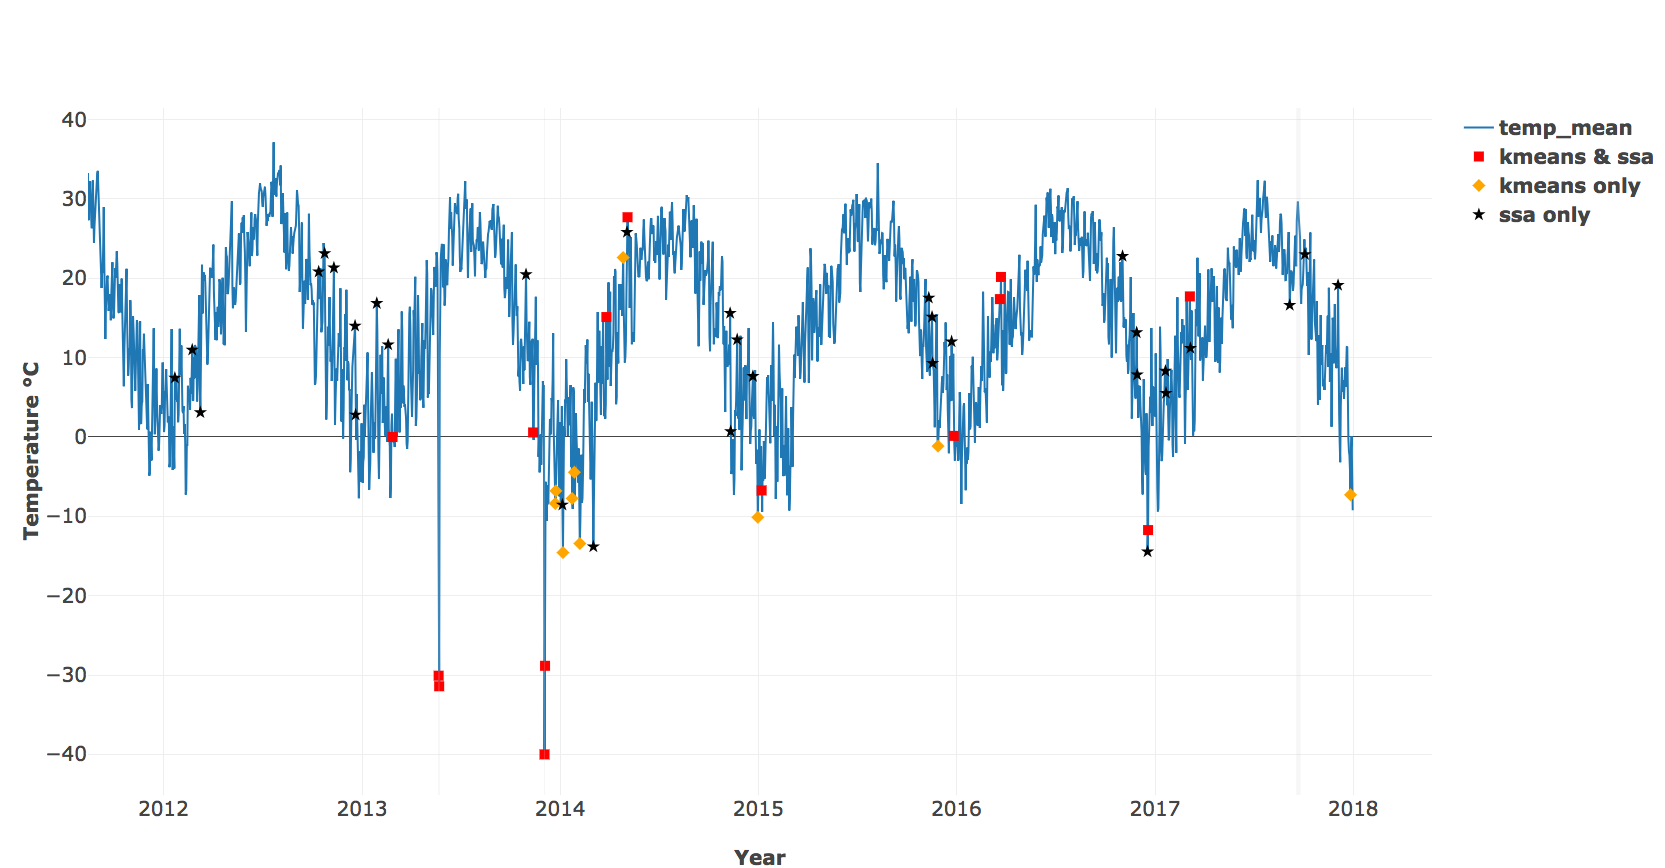
\includegraphics[width=\textwidth]{combined.png}
    \caption{Outliers detected for E33 \textit{temp\_mean} using combined algorithms}
    \label{fig:combined}
\end{figure*}

\begin{table}[ht]
\caption{Comparison of SSA and K-means Outlier Set Size}
\label{tab:comp}
\centering
\begin{tabular}{|l|c|}
\cline{2-2}
\multicolumn{1}{l|}{} & Outlier Set Size\\
\hline
SSA & 922\\
K-means & 508\\
Intersection & 378\\
Symmetric Difference & 674\\
\hline
\end{tabular}
\end{table}

\begin{table}[ht]
\caption{Precision and Recall of SSA and K-means}
\label{tab:pr}
\centering
\begin{tabular}{|l|c|c|c|}
\hline
Method & Variable & Precision & Recall\\
\hline
SSA & temp\_mean & 16.00\% & 1.20\%\\
SSA & vapor\_pressure\_mean & 20.70\% & 1.40\%\\
SSA & atmos\_pressure & 0.00\% & 0.00\%\\
SSA & rh\_mean & 14.80\% & 0.50\%\\
SSA & wspd\_arith\_mean & 0.60\% & 1.50\%\\
Kmeans & 5 together & 12.90\% & 1.90\%\\
Combined & 5 together & 11.10\% & 4.10\%\\
\hline
\end{tabular}
\end{table}

% DQR here
The current data quality or outlier detection is maintained as data quality reports (DQRs) stored in the DQR database with each entry manually entered \cite{mccord2016arm}. A description of an event which changed the normal data is included in these DQRs. The event could be temporary operating conditions such as power failures and frozen and snow covered sensors, instrument degradation, and contamination. It could also be an extreme weather event that has never been observed before. Each DQR entry also contains a specific time range affected, list of data projects, and specific measurements. And these entries are usually submitted by either the Data Quality Office \cite{peppler2016arm} or the instrument mentor \cite{cress2016deploying}. It is easy to notice that this method is not efficient as it requires a lot of labor. It is nearly also impossible to detect all the outliers due to the complexity and high volume of the ARM data.

Currently, not many outliers entries stored in DQR database. Here we used detected outliers in the DQR database as the ground truth to compare with the results from our framework. Precision and recall which were first defined in \cite{perry1955machine} were used as the comparison metric. They are commonly used to measure the quality of classification tasks \cite{olson2008advanced}. Precision is calculated from True Positives divided by the sum of True Positives and False Positives. On the other hand, recall is measured from True Positives divided by the sum of True Positives and False Negatives. We treated outliers in DQR database as True Positives. Thus detected outliers not in the DQR database are False Positives. Undetected values which in the DQR database are False Negatives, and which not in the DQR database are True Negatives. Table 3 contains the statistics of the comparison.

Precision attempts to answer What proportion of positive identifications was actually correct. The Combined precision is 11.10\% which shows that many outliers detected by the framework are not in the DQR database. Recall tries to solve What proportion of actual positives was identified correctly. The number is 4.10\% which is even smaller than precision. One reason is the same as precision that the size of True Positives is much small. The other reason is that DQR database records the whole possible affected time range which makes the size of False Negatives large. It could possible only a few days the data recorded are wrong.

\section{Conclusions}
In this paper we tested pairwise Pearson correlation coefficient, univariate SSA and multivariate K-means and combined them as a framework to detect outliers in the ARM data. Each method has its own drawbacks. But our experiments showed that this framework works well compared to the manually Data Quality Report method. Currently, we only tested MET data from SGP. And we analyzed data from each instrument independently. We'll apply this framework on other types of data from other facilities in the future. Meanwhile, other methods will be examined to test data from multiple instruments together such as graph theory methods \cite{phillips2015graph} and machine learning methods. 

%\addtolength{\textheight}{-12cm}  % This command serves to balance the column lengths
                                  % on the last page of the document manually. It shortens
                                  % the textheight of the last page by a suitable amount.
                                  % This command does not take effect until the next page
                                  % so it should come on the page before the last. Make
                                  % sure that you do not shorten the textheight too much.

%%%%%%%%%%%%%%%%%%%%%%%%%%%%%%%%%%%%%%%%%%%%%%%%%%%%%%%%%%%%%%%%%%%%%%%%%%%%%%%%
\section*{Acknowledgment}
This research was supported by the Atmospheric Radiation Measurement (ARM) user 
facility, a U.S. Department of Energy (DOE) Office of Science user facility 
managed by the Office of Biological and Environmental Research.


\bibliography{main} 
\bibliographystyle{IEEEtran}


\end{document}